\chapter{Hardware}

% % \ref{fig:coordination-diagram}.
 
\begin{figure} [H]
    \centering
    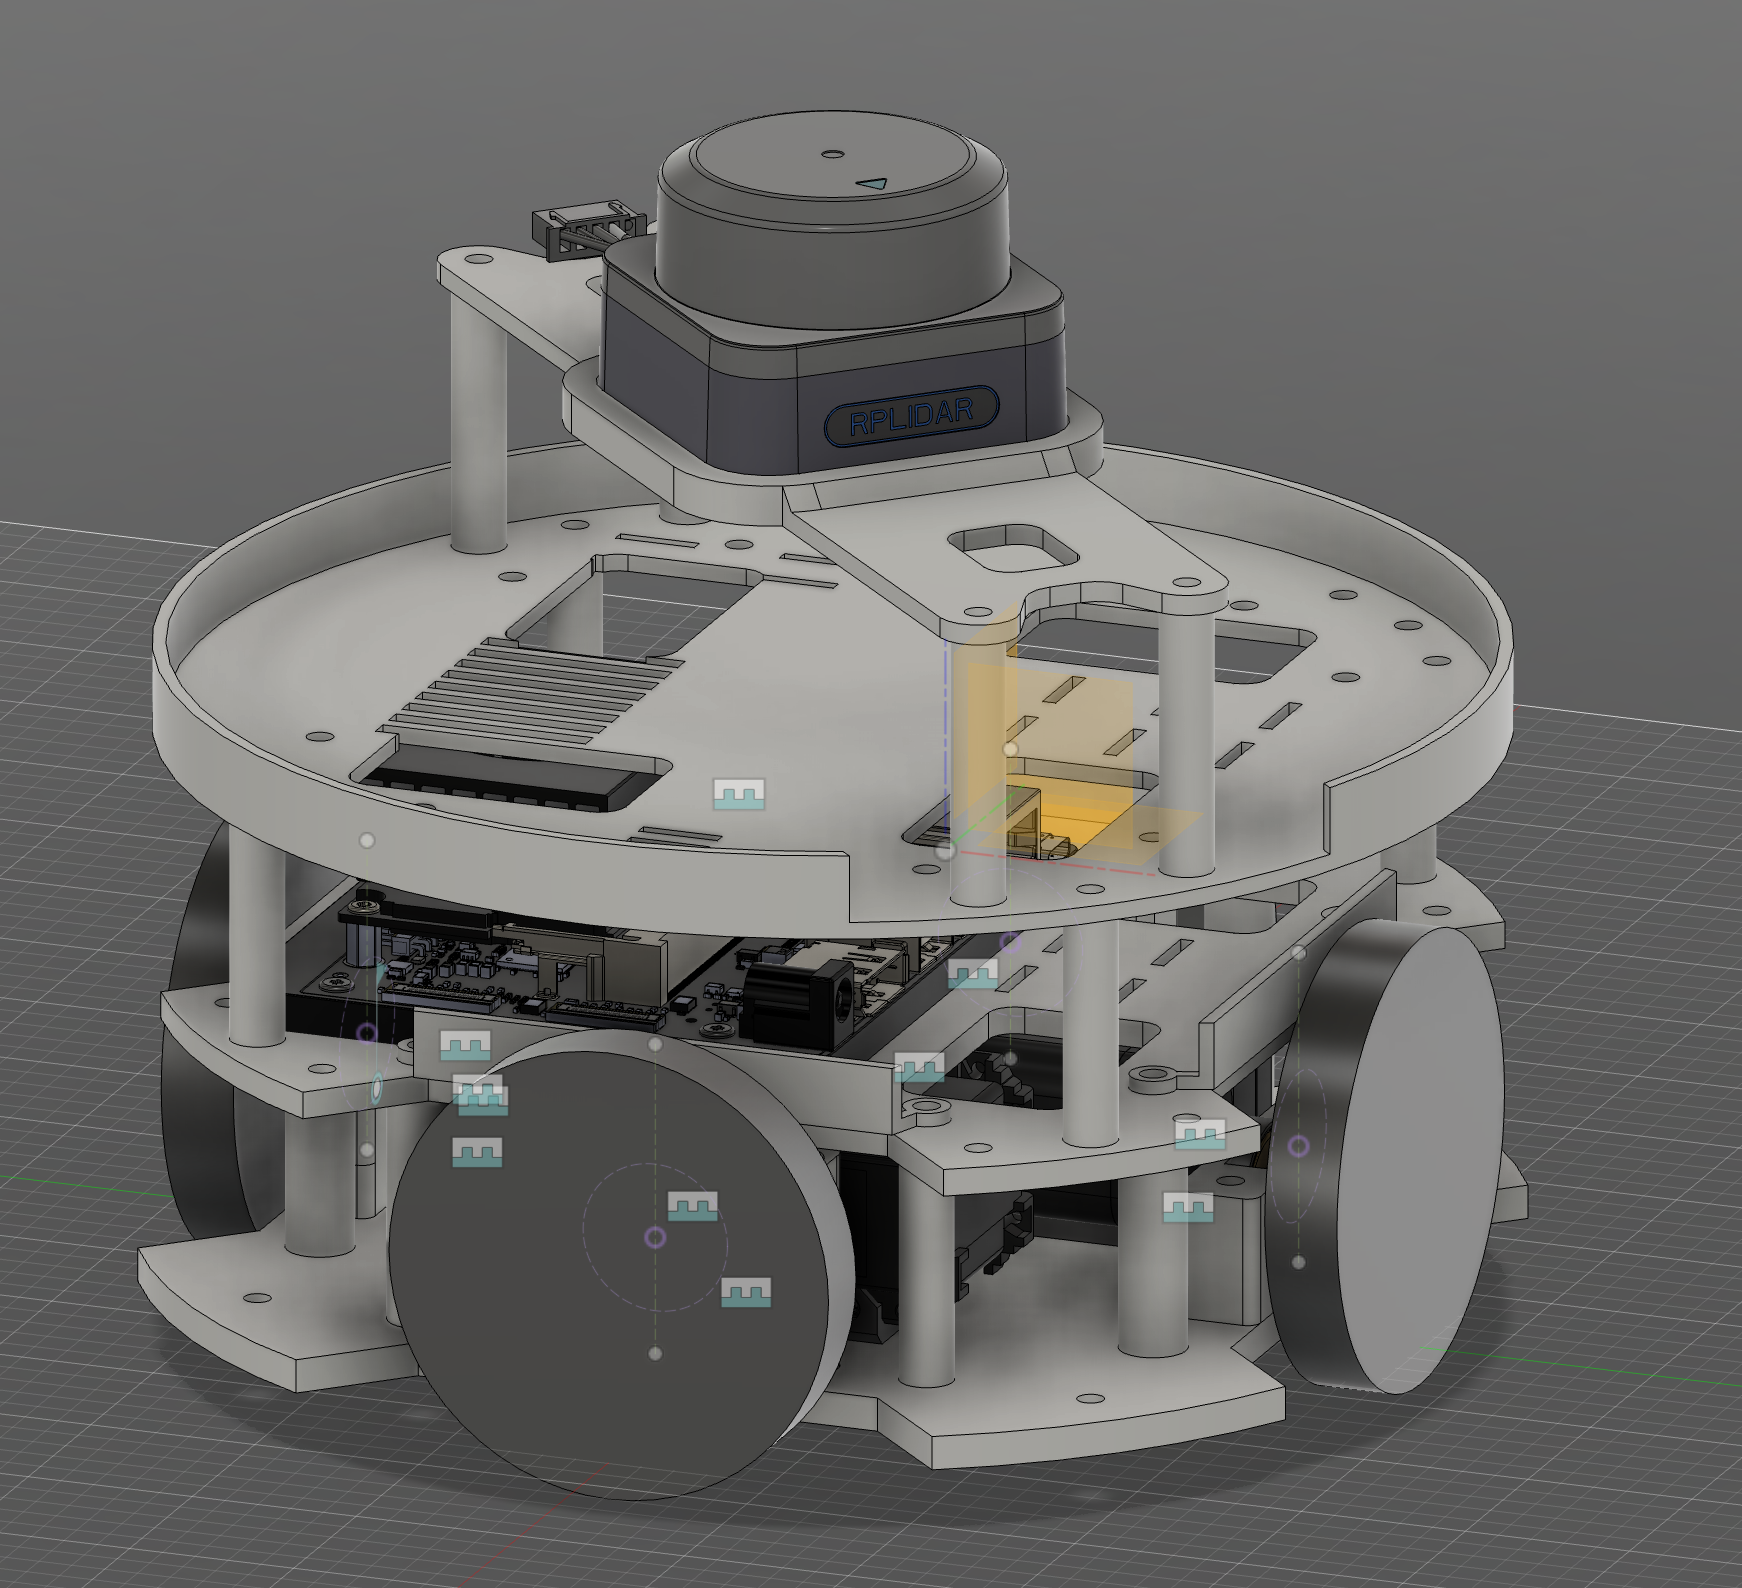
\includegraphics[width=0.65\linewidth]{assets/images/hardware/robotcad3layer.png}
    \caption{Robot CAD model}
    \label{fig:robo-cad}
\end{figure}

In this semester, we are testing our software on real hardware.  For the base of the robot, currently, we are using PLA using additive manufacturing method, Bambulab P1P with coreXY technology for rapid prototyping, the entire robot including: the base, shaft, flange coupler, bearing holder, standoff, plate for different floor of the robot, the mount for the LiDAR, were all printed, which takes around 12 hours per robot. All the parts was able to be printed with a tolerance of 0.1mm. However, we planned to change the baseplate to acrylic for increased the stiffness and the flatness of the base to increase the grip of the wheel of the robot. In additional to the plate, the shaft, wheel, and flange coupler for the motor will be changed from PLA to stainless steel 304 for durability and reduce tolerance.
The model of the robot for 3D printing can be seen in the figure 
The model of the robot is a X-Drive 45 degrees, which is a holonomic robot with 4 wheels, each wheel is driven by a motor.

\begin{figure} [H]
    \centering
    \includegraphics[width=0.65\linewidth]{assets/images/hardware/irlrobotv1.png}
    \caption{Robot Prototype}
    \label{fig:robo-irl}
\end{figure}

The motors of the robot are the Dynamixel AX-12W with a low gear ratio to increase the back drivability of the system as each wheel are angled at 45 degrees. The motor is a servo with wheel mode, which allows the motor to rotate 360 degrees continuously. The motor is controlled by a motor driver using Python SDK; said SDK are used in a custom ROS package which include the transform of the high-level Twist message which contain linear and angular velocity to the 4 motor in the X-Drive 45 degrees orientation. We utilized Jacobian matrix to transform the Twist message to the motor velocity. The equation of the transfer was aided by KMUTNB \cite{phunopas2018motion}

We have moved from using the 20 years old Maxon BLDC with the XDrive as we have found that the motor is not suitable for the XDrive as there's a lot of unnecessary work which needs to be done such as retrofitting new encoders to each motor. Time which will better utilized in developing the software to focus on the main goal of this project which is the software layer of coordinating the robot together.

\begin{figure} [H]
    \centering
    \begin{tabular}{@{}c@{\hspace{0.3cm}}c@{\hspace{0.3cm}}c@{}}
        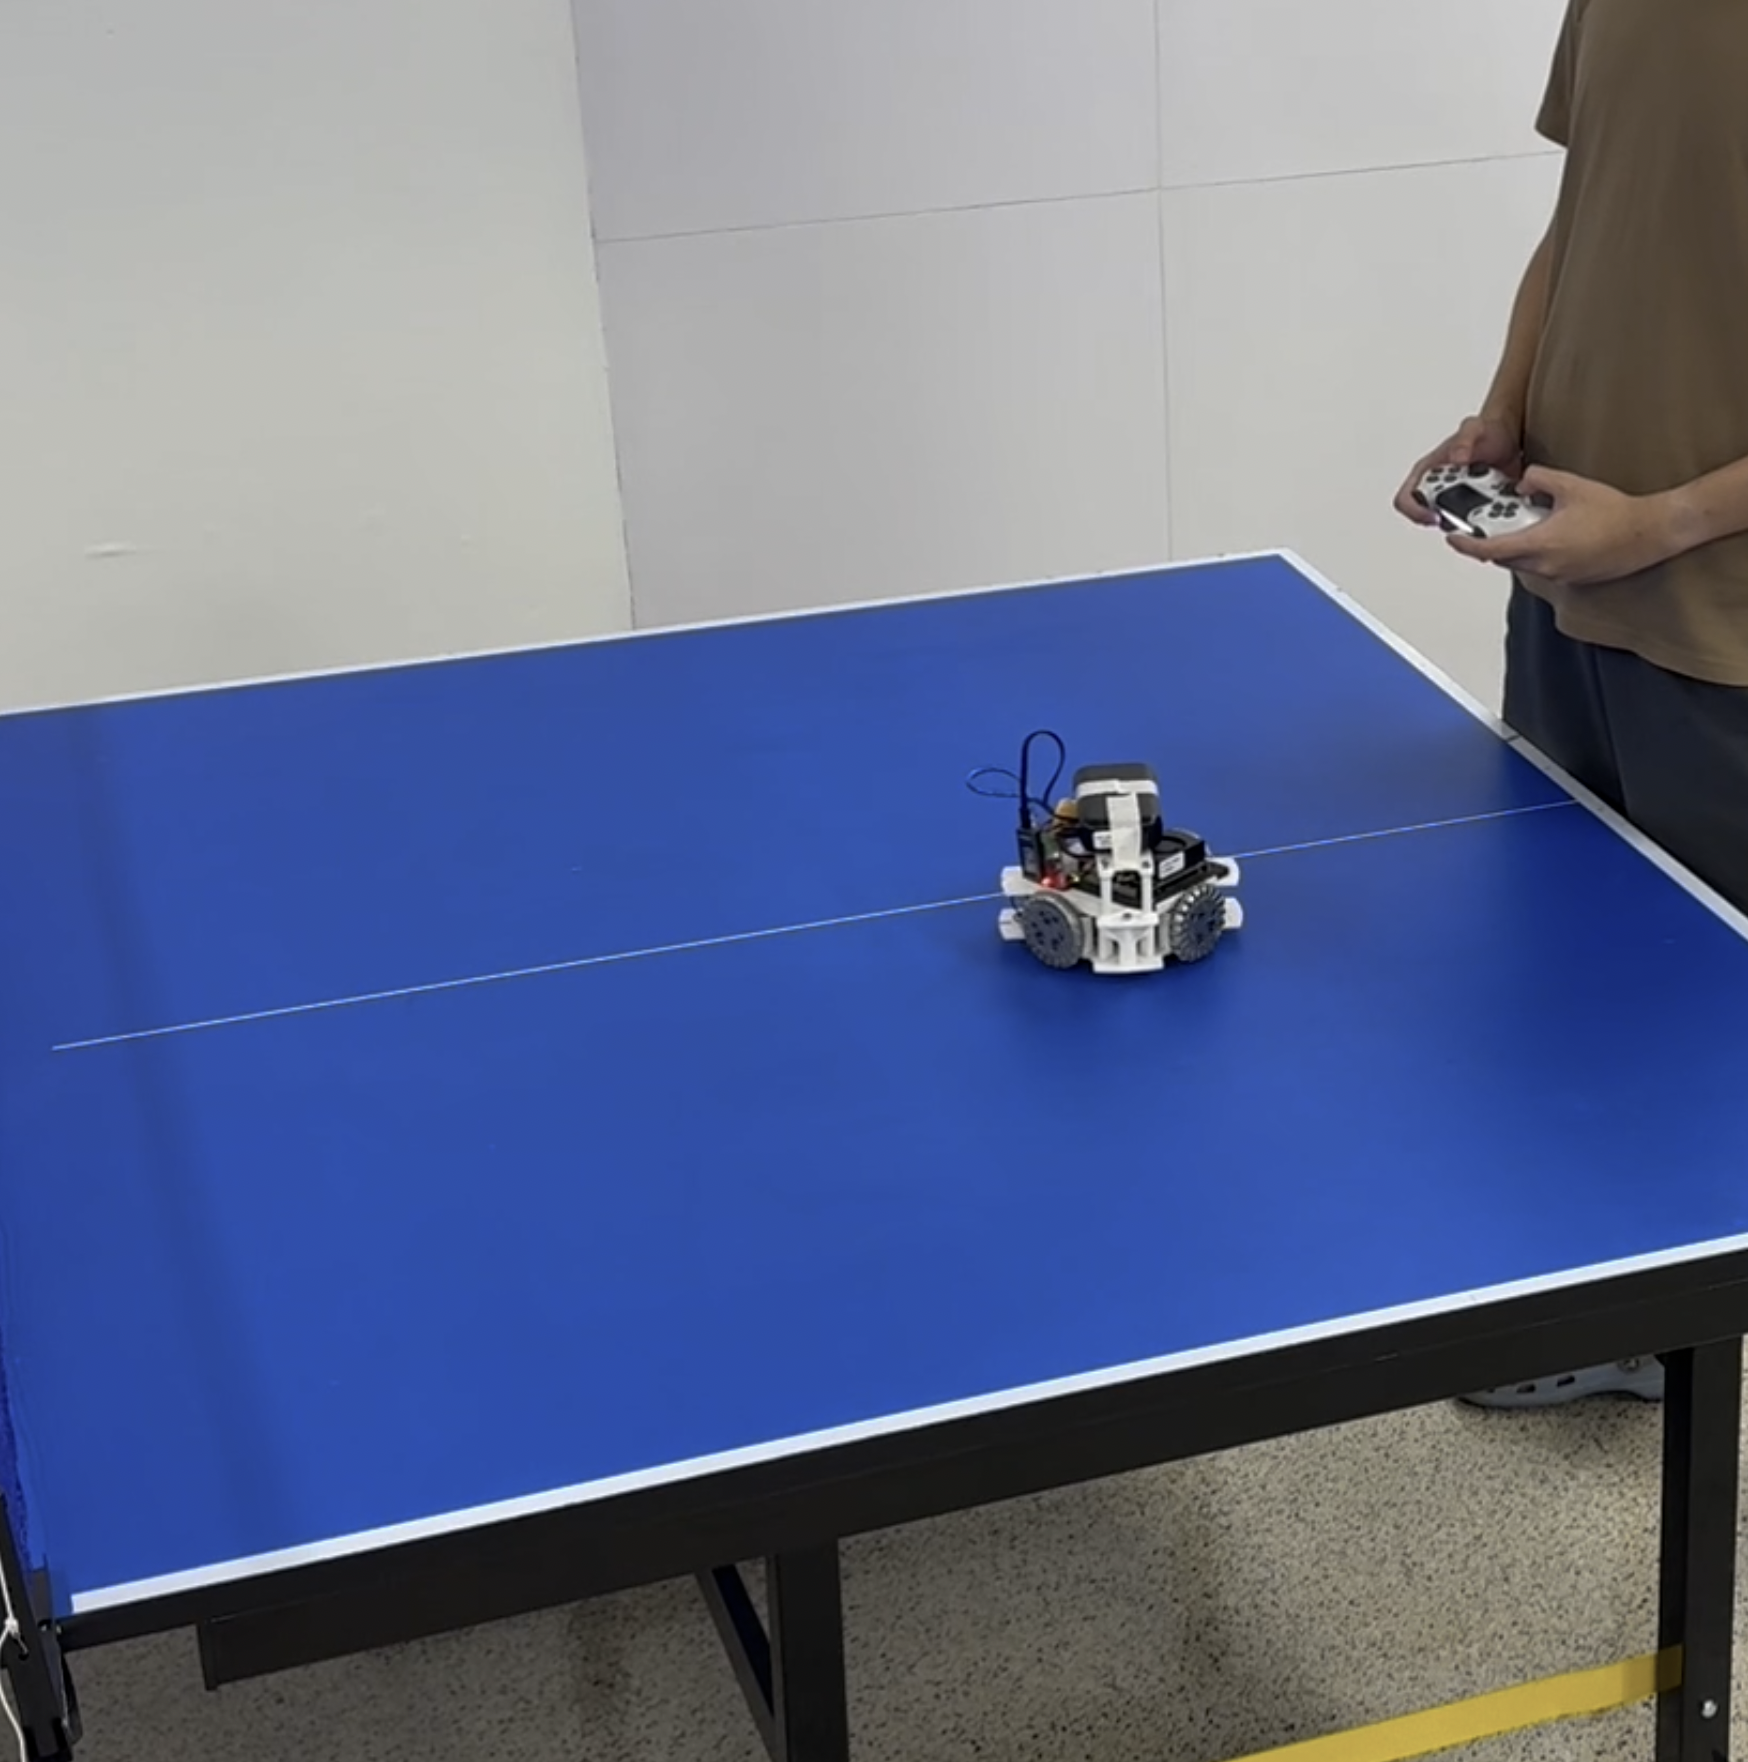
\includegraphics[width=0.3\textwidth]{assets/images/hardware/move1.png} &
        \includegraphics[width=0.3\textwidth]{assets/images/hardware/move3.png} &
        \includegraphics[width=0.3\textwidth]{assets/images/hardware/move2.png} \\
        \small frame 1 &
        \small frame 2 &
        \small frame 3 \\
    \end{tabular}
    \caption{Holonomic movement capabilities of the robot}
    \label{fig:holo-movement}
\end{figure}

The work described in this section has lead to robot successfully to move holonomically with the freedom of moving in any direction in the XY plan of the floor. The figure \ref{fig:holo-movement}. attached illustrates the movement of the robot being controlled with teleop\_keyboard package in ROS2 Humble. Later in this report we will report on the geometry of the robot and the current limitation of the robot and the plan to overcome the limitation of the robot.